\section{Measuring}

\begin{frame}
\frametitle{Time measurement equipment: hardware}
\begin{itemize}
\item The best equipment is an oscilloscope.
\item Allows to time the "Power on" event (connected to a power rail),
      or any event (connected to a GPIO pin, for example), all this
      in a very accurate way.
\item Easy to write to a GPIO at all the stages of system booting.
\item Some oscilloscopes are getting affordable. Example: Bitscope
      Pocket Analyzer (295 AUD, supported on Linux, \url{http://www.bitscope.com/product/BS10/})
\end{itemize}
\begin{center}
    % From http://openclipart.org/detail/28033/oscilloscope-by-mothinator
    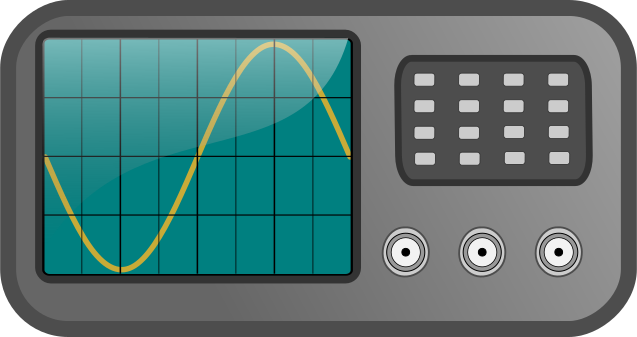
\includegraphics[width=0.35\textwidth]{slides/boottime-measuring/mothinator_Oscilloscope.pdf}
\end{center}
\end{frame}

\begin{frame}
\frametitle{Time measurement equipment: serial port}
\begin{columns}
\column{0.75\textwidth}
\begin{itemize}
\item Useful when you don't have an oscilloscope, or don't want to make
      take any risk connecting wires to the hardware.
\item Usually relies on software which times messages received from the board's
      serial port (serial port absolutely required). Such software
      runs on a PC connected to the serial port.
\item Need a real serial port (directly connected to the CPU),
      immediately usable from the earliest parts of the boot process.
\item Limitation: won't be able to time the "Power on" event in
      an accurate way. But acceptable as you can assume that
      the time to run the first stage bootloader is constant.
\end{itemize}
\column{0.25\textwidth}
% From http://openclipart.org/detail/173570/serial-db9-female-by-deusinvictus-173570

\includegraphics[width=\textwidth]{slides/boottime-measuring/serial_db9_female.pdf}
\end{columns}
\end{frame}

\begin{frame}
\frametitle{Time measurement equipment: USB to serial}
\begin{columns}
    \column{0.65\textwidth}
	\begin{itemize}
	\item Serial ports over USB {\bf device} are fine if there's an on-board
	      serial-to-USB chip directly connected to the CPU serial port (very frequent).
	\item Attaching a USB-to-serial dongle to a USB {\bf host} port on
	      the device won't do: USB is available much later and messages
	      go through more complex software stacks (loss of time accuracy).
	\item All development boards have a standard or USB serial port.
	\end{itemize}
    \column{0.35\textwidth}
	% From http://openclipart.org/detail/135721/usb-cable-by-gsagri04
	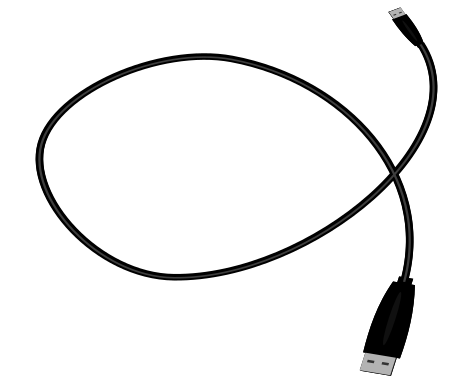
\includegraphics[width=\textwidth]{slides/boottime-measuring/GS_USB_Cable.pdf}
\end{columns}
\end{frame}

\begin{frame}
\frametitle{grabserial}
\begin{itemize}
\item From Tim Bird: \url{https://elinux.org/Grabserial}
\item A Python script to add timestamps to messages coming from a
	serial console.
\item Key advantage: starts counting very early (bootstrap and bootloader)
\item Another advantage: no overhead on the target, because run on the host machine.
\item Drawbacks: may not be precise enough. Can't measure power up time.
\end{itemize}
\end{frame}

\begin{frame}
\frametitle{Using grabserial}
\begin{center}
    \includegraphics[height=0.65\textheight]{slides/boottime-measuring/using-grabserial.pdf}
\end{center}
{\small
{\bf Caution}: \code{grabserial} shows the arrival time of the
{\bf first character} of a line. This doesn't mean that the entire line
was received at that time.}
\end{frame}

\setuplabframe
{Measuring}
{
\begin{itemize}
\item Time the various components of boot time
\end{itemize}
}
